\Section{The Goman and Khrabrov model}

\Subsection{Motivation}
In their 1994 paper entitled ``State-Space Representation of Aerodynamic Characteristics of an Aircraft at High Angle of Attack'' \cite{GK} Goman and Khrabrov introduce a new model for characterizing the lift and moment coefficients for slender delta wings.
Their goal was to study the stability of delta wing fighter jets where maneuverability is important, and to link it to physical fluid dynamic phenomena such as vortex breakdown or flow separation.

\par The classical stability analysis method relies on a Taylor series expansion of the aerodynamic coefficients.
% maybe put an example here.
This linear representation is relatively accurate for fully attached flows but the model breaks down at higher angles of attack when separation occurs.
In the semi-separated region the aerodynamic effects are mainly driven by the degree of flow separation happening on the wing.
For this reason they chose to define $C_l$ as a function of $\alpha$, the angle of attack, and a state variable $x$ representing the degree of separation.
This degree of separation can be defined as the position of the vortex breakdown point if you are looking at delta wings, or the position of the reattachment point in the case of 2D airfoils.
This allows for a model tightly defined by the physics of the flow.


\Subsection{Flow physics and state variables}
Since this study was performed with a 2D NACA0009 airfoil, we define the state variable $x$ as the position of the reattachment point.
Its value changes from 1 when it is situated at the leading edge to 0 when it gets to the trailing edge and beyond.
For quasi-steady cases the separation point is a function of the angle of attack. If we define $x_0$ as the separation point position in a quasi-steady situation then

\begin{equation}
  C_l^{qs} = f(\alpha,x_0(\alpha))
  \label{eqn:qs_Cl}
\end{equation}

The unsteady part of the flow physics can be divided into two groups of phenomena.

\par The first are the effects of the pitch rate, $\dot{\alpha}$, on the position of the separation point.
Goman and Khrabrov argue that this is roughly proportional to the pitch rate $\dot{\alpha}$, and as such, they can be included by modifying the quasi-steady state value by using $x_0 (\alpha - \tau_2 \dot{\alpha})$ 

\par The second phenomenon is due to the dynamics of the separated flow.
The flow has a certain relaxation characteristic under a disturbance input.
This can be modeled using a first order differential equation.

\begin{eqnarray}
  \tau_1 \frac{dx}{dt} +x = x_0(\alpha - \tau_2 \dot{\alpha}) 
  \label{eqn:state_variable}
\end{eqnarray}

This model will be tested with experimental data.

\Section{Experimental Setup}

\Subsection{Equipment and facilities}

\begin{figure}[h]
  \begin{center}
%\includegraphics{<+file+>}
  \end{center}
  \caption{Airfoil model inside the wind tunnel}
  \label{fig:wind_tunnel}
\end{figure}

The experimental part of this research was performed in the Andrew Fejer Unsteady Wind Tunnel at the Illinois Institute of Technology, Chicago.
This is a low velocity wind tunnel with a 60cm by 60cm test section.
The wind tunnel is mainly used for unsteady aerodynamic studies.
Airfoils are mounted on a motorized sting outfitted with two linear electric servo-motors.
These servos are powered by an amplifier with a integrated PID system and driven by an analog voltage input signal proportional to the desired position.

\begin{figure}[h]
  \begin{center}
%		\includegraphics{<+file+>}
  \end{center}
  \caption{Pitching and plunging mechanism}
  \label{fig:pitching_mechanism}
\end{figure}

As seen on figure \ref{fig:pitching_mechanism} combining the motion of the front and back servo allows for the wing to be plunged as well as pitched around a range of axes.
The tunnel is also equipped with a system of shutters that can be used to create wind gusts.
However this feature will not be used in this project.

\par The input signal for the servos is made with Simulink\textsuperscript{\textregistered} and fed through D-Space\textsuperscript{\textregistered} to produce a control voltage for the servo tubes. 

\par Several sensors are used for data acquisition.
A pair of linear potentiometers measures the position of the servos in order to determine the airfoil pitch angle.
The flow speed is measured via a Pitot tube and pressure transducer plugged into a acquisition box.
In parallel to this acquisition system the forces exerted on the airfoil can be measured.
A piezoelectric ATI Nano17 force balance is located between the sting and the airfoil.
This sensor measures both absolute forces and moments along 3 different axis.

\par The wing is made out of balsa wood with the structure wrapped in monocote, a heat-shrunk plastic film.
Its chord length is 245mm and its width 560mm with a NACA0009 profile.
It connects to the force balance at a point at 25 percent of the chord.
The design was made to keep the weight and moment of inertia as small as possible to minimize the inertial effects when the wing is moving.


\FloatBarrier

\Subsection{Experimental procedure and data processing}
Different pitch input amplitudes have been tried.
There was some concern that if the pitching axis wasn't on the axis symmetry, at the quarter chord of the airfoil, additional aerodynamic phenomenon would affect the data.
After testing different pitching input that placed the rotation axis either at the top of the front servo, at the top of the force balance or at the top of the back servo,  it was determined that the optimal way to drive the pitching mechanism was to move only the back servo.
Other input methods induced too much mechanical vibrations.

\par The amplifier driving the electric servos has its own PID control system, however even after careful tuning some error exists between the commanded angle of attack and the actual angle of attack.
To negate that effect the actual servo position, as given by the potentiometers, is used for our measurements.
This data is used to transform the normal and tangent force into lift and drag (via a simple rotation matrix). 
They are then normalized (divided by $\frac{1}{2}\rho S U^2$, with $S$ the surface area of the wing, $\rho$ the air density and $U$ the free stream velocity) to get the aerodynamics coefficients.

\par Unless specified otherwise, all the acquisitions have been done at a flow speed of 3m/s which correspond to a chord based Reynolds number of 50000.

\par For each experimental case the force balance as well as the servo position and a synchronization signal are simultaneously acquired.
A first offset with the tunnel off and the wing pitching is taken to let us get the force balance offset as well as record the inertial effects.
Even though the wing only weighs around 300 grams, these inertial effects represent the majority of the forces measured by the force balance.
Moreover some of the force measured come from the springiness of the cables used for the active flow control part.
After the first offset the real case is taken, followed by a second offset to account for the drift in the force balance measurement sometime seen over the course of several minutes.

\par During each acquisitions at least 50 cycles are recorded.
This allows us to perform phase averaging.
Phase averaging is done by slicing the files into individual cycles (thank to the synchronization signal) and then making an average of these cycles.
With this technique the signal to noise ratio of greatly improved.
Once this has been done with the two offsets and the proper acquisition itself, aerodynamic forces are obtained by subtracting the offsets.
All processing is done with Matlab\textsuperscript{\textregistered}. 

\par The servo actuation system has a small but noticeable dead band as well as a delay between the input and output.
This makes the actual pitching motion slightly different from the input.
To account for the dead band the actual measured pitch angle is used as an input of the GK model when we want to compare its prediction with the experimental data.

\par Finally the GK model itself is also implemented in Matlab.
The code can be seen in Appendix \ref{ch:GK_code}.



\FloatBarrier


\Section{Adapting the GK model to the NACA0009}

\Subsection{Steady lift and stalling behavior}
With the basics of the GK model defined, the goal is now to adapt it to our objectives.
If this model is to be used for optimization purposes the drag also needs to be calculated.
The original model defined by Goman and Khrabrov included the lift and pitching moment coefficients.
Similar to their model the assumption is made that the lift and drag coefficients share the same state variable.
As such we define $f$ and $g$ as

\begin{equation}
  \begin{array}[c]{c}
    C_l=f(\alpha,x) \\
    C_d=g(\alpha,x)
  \end{array}
  \label{eqn:lift_drag_functions}
\end{equation}

\par The other difference with their case study is that we are considering a 2D airfoil whereas they modeled a 3D delta wing.
This means that we can not reuse the same lift function $f$ as the original paper.

\par In order to get an accurate equation for the lift and drag, a quasi-steady map of the lift and drag coefficients is made.
This map is done by very slowly (0.1 degree per seconds) pitching the wing between -5 and 25 degrees.
The free stream speed has to be corrected to account for the flow slowing down during the higher blockage ratio at high angle of attack.

\begin{figure}[ht]
  \begin{center}
    \scalebox{1.0}
    {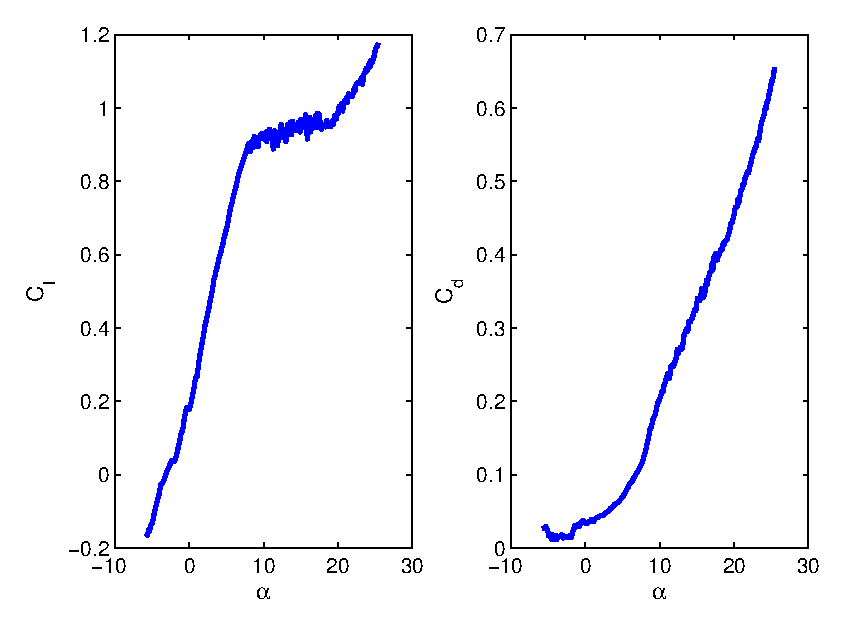
\includegraphics{./Figures/Cd_and_Cl_NACA0009.eps}}
  \end{center}
  \caption{Lift and drag coefficient in the quasi-steady case}
  \label{fig:QS_Cl_Cd_vs_alpha}
\end{figure}

\par Figure \ref{fig:QS_Cl_Cd_vs_alpha} shows how the aerodynamics behave for our NACA0009 airfoil.
The lift coefficient is close to a clean linear function when the flow is attached.
The separation begins around 8 degrees, and the lift coefficient remains constant in the 10 to 20 degrees zone when the flow is partially separated.
At higher angle of attack the flow is totally separated and $C_l$ is once again proportional to $\alpha$ but with a different slope this time.
Even though the NACA0009 has a symmetric profile, the measured lift coefficient for a angle of attack of zero is not null.
It is suspected that the sting onto which the airfoil is fixed may disturb the flow and cause this asymmetry.
Moreover this curve differs slightly from the ones found in the literature.
Once again this can be attributed to the experimental setup.
Other than the sting effects the couple of millimeters of clearance between the wall of the wind tunnel and the edge of the airfoil are probably to blame as they induce some 3D effects.
These gaps are necessary to allow for the both pitching and plunging of the wing.

\par From the static map we can approximate the part where the flow is still attached (<8 degrees) by 

\begin{equation}
  \begin{array}[c]{c}
    C_l= 2 \pi \cdot \alpha + C_{l0} \\
    C_d= \frac{C_l^2}{2G_{max}} + C_{d0}
  \end{array}
  \label{eqn:attached_Cl_and_Cd_vs_alpha}
\end{equation}

Which is remarkably close to the classical theoretical result for a 2D airfoils in a ideal inviscid attached flow.

\Subsection{State variable approximation}
When the flow is still attached the value of $x$ is 1, which means that we are considering the separation point to be at the trailing edge.
Similarly when the flow is totally separated the separation point is at the leading edge and $x=0$.
Since for totally separated flow the slop of the lift coefficient as a function of $\alpha$ can be approximated to about $0.4$ of the slope for the attached flow, we choose to use the following equation for the lift over the whole range of angle of attack. 

\begin{equation}
  C_l(\alpha,x)=2 \pi \cdot \alpha (0.6 x + 0.4) + C_{l0}
  \label{eqn:Cl_function}
\end{equation}

\par By inverting this equation the value of $x_0$ can then be adjusted so that the output of this function matches the experimental data. 
The resulting profile for $x_0(\alpha)$ can be seen in figure \ref{fig:x_0_vs_alpha}

\begin{figure}[h]
  \begin{center}
    \scalebox{1.0}
    {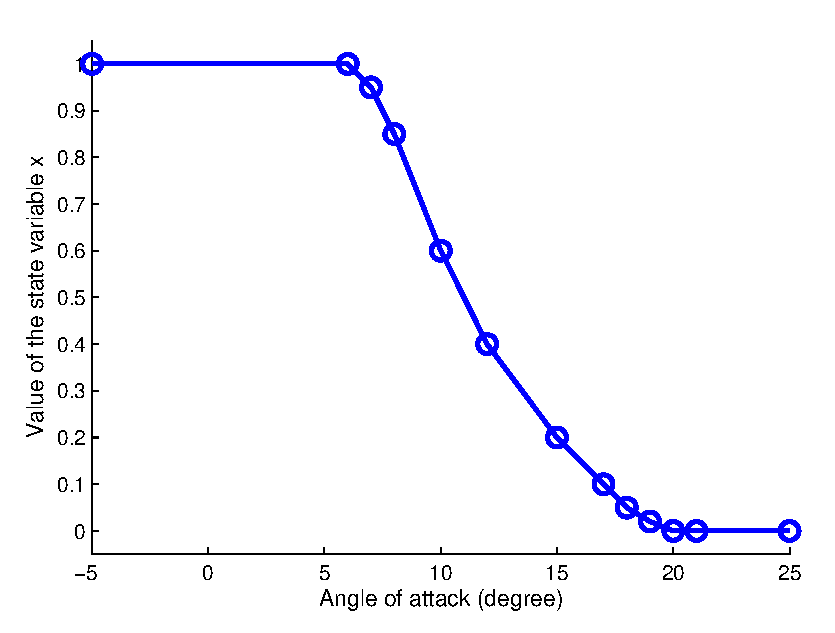
\includegraphics{./Figures/x_0_vs_alpha.eps}}
  \end{center}
  \caption{Quasi-steady profile for the state variable $x$}
  \label{fig:x_0_vs_alpha}
\end{figure}

\FloatBarrier
With this profile we get a good approximation of the experimental $C_l(\alpha)$ (cf figure \ref{fig:GK_Cl_vs_alpha}) for quasi steady cases.

\begin{figure}[h]
  \begin{center}
    \scalebox{1.0}{
      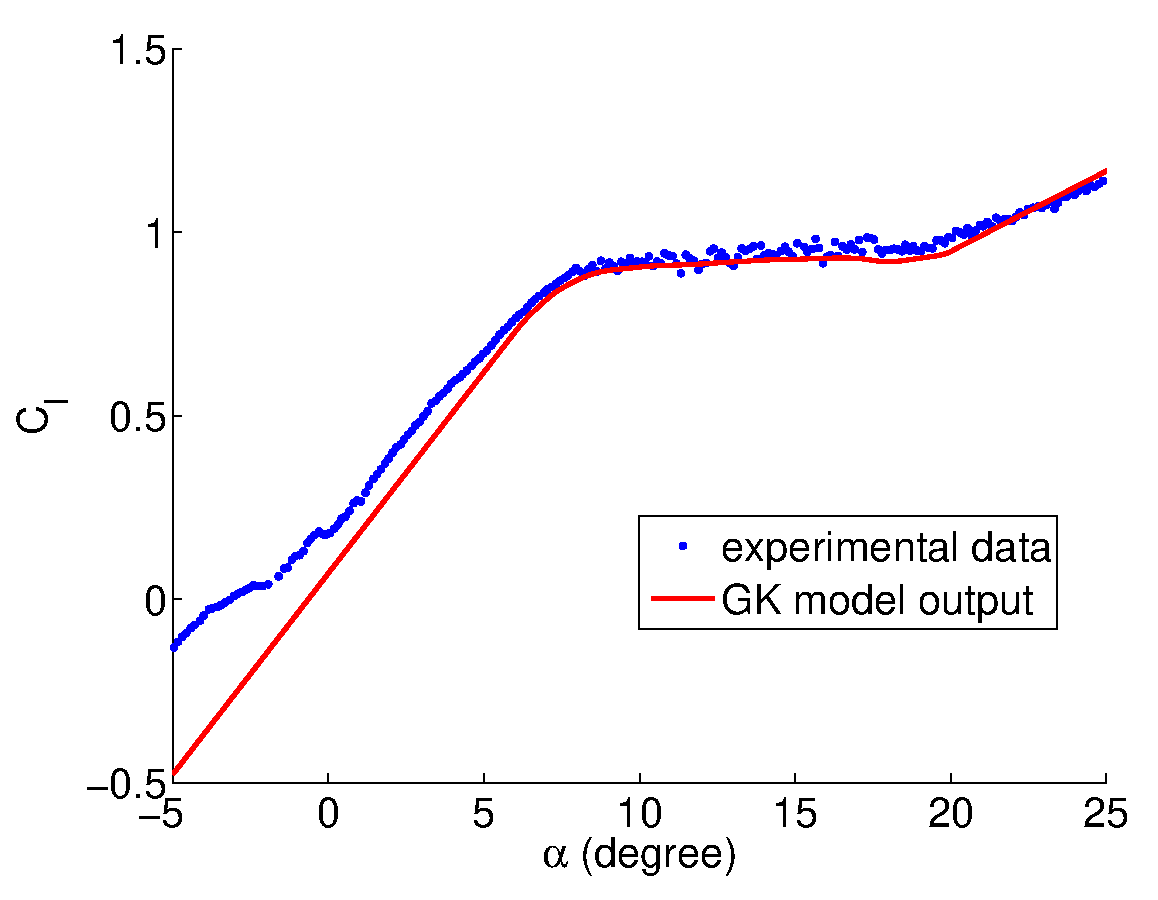
\includegraphics{./Figures/GK_cl_vs_alpha.eps}}
  \end{center}
  \caption{Comparison between the experimental and model quasi-steady lift}
  \label{fig:GK_Cl_vs_alpha}
\end{figure}

\par The assumption that the drag shares the same state variable as the lift is confirmed when the following equation produces similarly accurate results compared to experimental data, as seen on figure \ref{fig:GK_Cd_vs_alpha}.

\begin{equation}
  C_d(\alpha,x)= \frac{ \left( \left( 2 - x \right)C_l \right)^2 }{2 G_{max}} + C_d0
  \label{eqn:Cd_function}
\end{equation}

\begin{figure}[h]
  \begin{center}
    \scalebox{1.0}
    {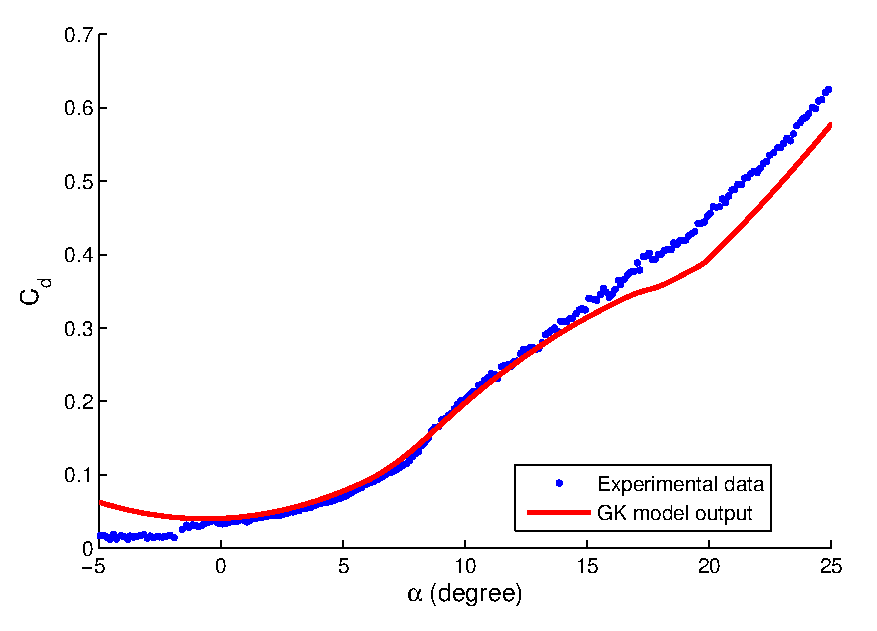
\includegraphics{./Figures/GK_cd_vs_alpha.eps}}
  \end{center}
  \caption{Comparison between the experimental and model quasi-steady drag}
  \label{fig:GK_Cd_vs_alpha}
\end{figure}

\par The $2\pi\alpha$ slope is a good first aproximation of lift coefficient slope.
However for a real airfoil the slope is usually less than this theoretical value.
To correct this a better coefficient can be found by averaging the slope of $C_l$ between 0 and 5 degrees of angle of attack.
Then the slope for angles of attack larger than 20 degrees must be taken into account to make sure the value of the state variable will converge to 0.
From there the same procedure of inverting the lift coefficient function can be used to get the quasi-steady $x$ curve.

\par These two relatively simple equations show that a physics-based GK model can be implemented for both lift and drag, and that they indeed depend on the same state variable.
The two time constants $\tau_1$ and $\tau_2$ will be determined in the next section when the wing undergoes unsteady pitching.

\FloatBarrier

\Subsection{Correlation between the state variable and the pressure surface}
In their paper Goman and Khrabrov \cite{GK} mention that the state variable should reflect the position of the separation point, but they show little evidence of this theory.
To check this assumption a wing model fitted with pressure sensors is used to map the position of the separation point for the quasi-steady map.

\par This airfoil has an array of 6 sensors situated on the top surface.
One additional sensor is fitted on the bottom of the wind tunnel to get the static pressure of the free stream.
These sensors measure the differential pressure between the measuring point and the lab pressure.

\begin{figure}[h]
  \centering
  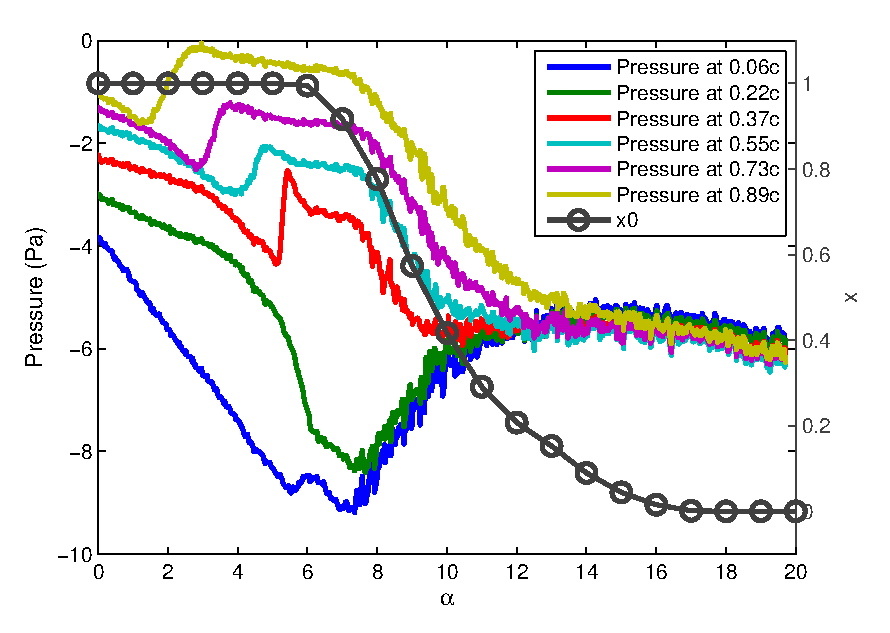
\includegraphics{./Figures/NACA0012_pressure_x0_vs_alpha.eps}
  \caption{Pressure relative to the position on the wing for the quasi-steady map}
  \label{fig:P_diff}
\end{figure}

\par As seen in figure \ref{fig:P_diff} the identification of the separation point isn't obvious.
There is clearly some sort jumps in the pressure that we can see creeping up from the trailing edge of the airfoil.
However this jump happens at angles where the lift coefficient is still linear with respect to the angle of attack.

\par For higher angles of attack the pressure data is even harder to interpret.
Something happens around 8 to 10 degrees for the pressure close to the leading edge but it is hard to correlate it to any feature on the state function.

\par From these results it is clear that inferring $x$ from the pressure would require a more in depth analysis of the pressure distribution on the airfoil.
Some work has been and is still being conducted on linking POD decomposition of the pressure to the lift forces but so far no definitive results seems to emerge.


\Section{Model validation}

\Subsection{Time constants}
While the ability to predict lift and drag based on separation can be useful, the real strength of the GK model resides in its ability to match the unsteady cases.
The first step is to determine the two time constants $\tau_1$ and $\tau_2$. 
To do that a series of pitching cases are performed. 
The pitching inputs are the following

\begin{equation}
	\alpha\left( t \right)= A \sin \left( 2 \pi \frac{t}{f} \right) + \alpha_0
	\label{eqn:pitch_input}
\end{equation}

With $A=2^\circ$ and $\alpha_0=12^\circ$.
The frequency $f$ is set to 0.25, 0.5, 1 and 2 Hz (respectively K of 0.064, 0.128, 0.257 and 0.513)

\begin{figure}[h]
  \begin{center}
    \scalebox{1.0}  
    {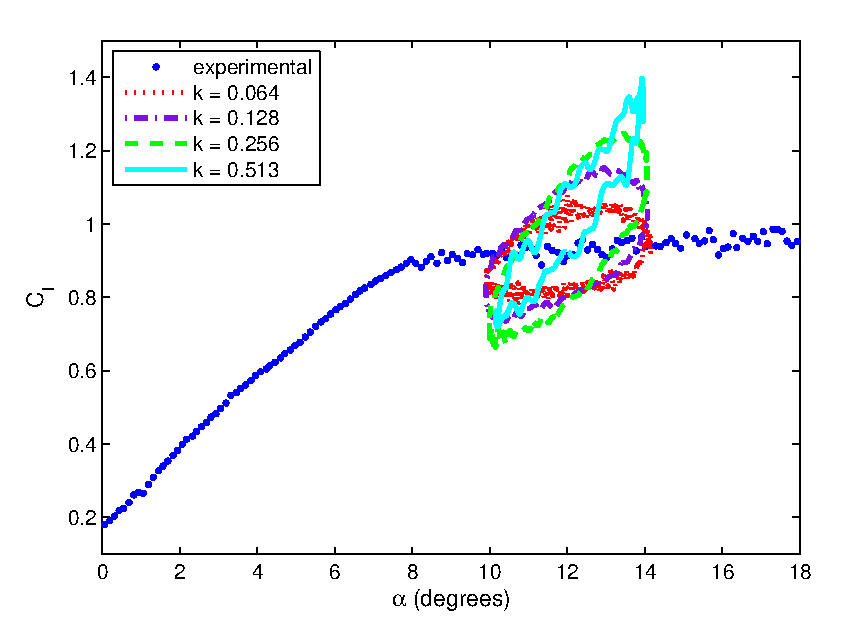
\includegraphics{./Figures/Pitching_allcases_CL_12_amp_2.eps}}
  \end{center}
  \caption{Unsteady effects on the lift of sinusoidal pitching around 12 degree} 
  \label{fig:Pitching_allcases_Cl_12}
\end{figure}

\begin{figure}[h]
  \begin{center}
    \scalebox{1.0}  
    {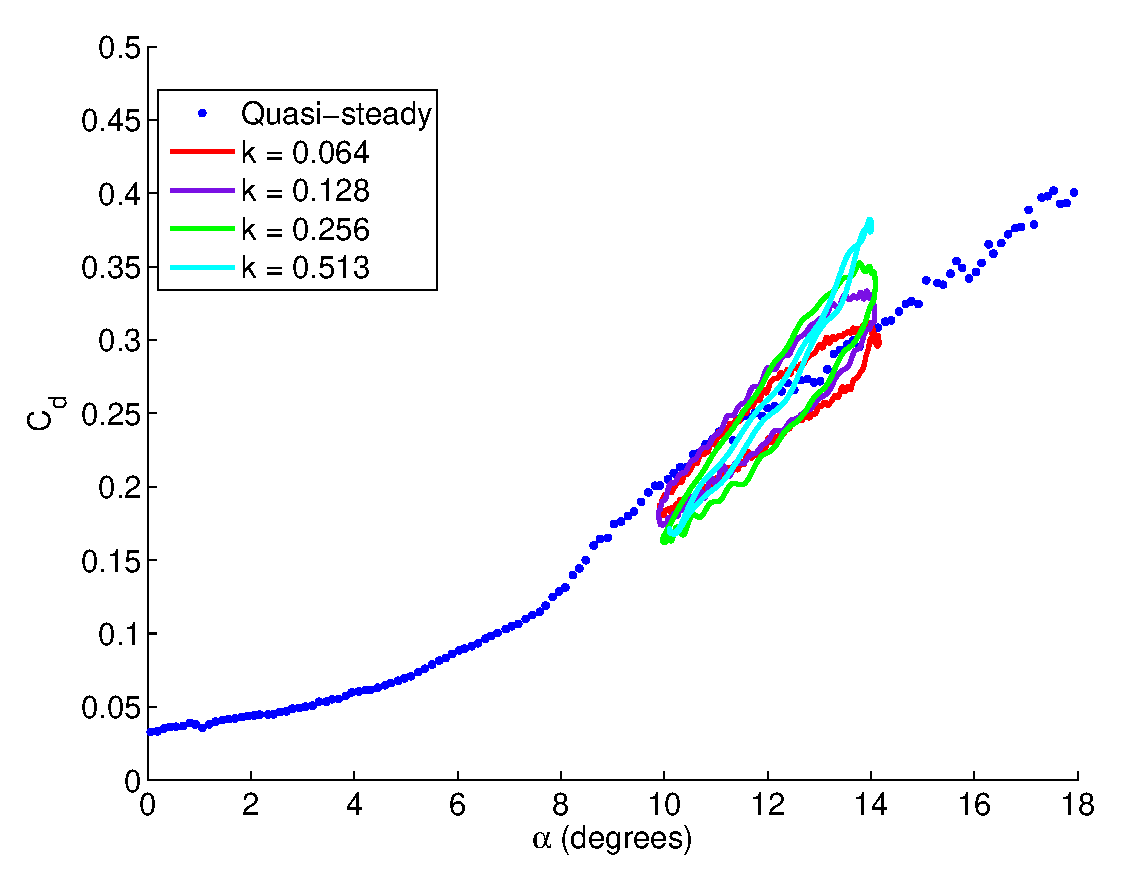
\includegraphics{./Figures/Pitching_allcases_CD_12_amp_2.eps}}
  \end{center}
  \caption{Unsteady effects on the drag of sinusoidal pitching around 12 degree} 
  \label{fig:Pitching_allcases_Cd_12}
\end{figure}

\FloatBarrier

\par On these figures it is easy to notice the influence of the time delays on the aerodynamic coefficients.
At the lower frequencies the loops are quite open and a significant difference exists between the lift obtained during the pitch up and the pitch down phase.
The lift values circulate on these loops, rotating in an anti-clockwise direction.
This means that the lift is higher during pitch down maneuver.
In contrast this behavior disappears at higher frequencies.
For $k$ values of 0.257 and 0.513 the difference between the pitch up and pitch down is lower.
However the lift variation amplitude is more pronounced in those cases.

\par Before using the GK model as a predictive tool, the time constants need to be found.
This is done by trial and error.
The two time constants are determined manually, and are tuned to produce the best results at the different frequencies tested.
$\tau_1$ is found to be equal to 3.06 t+ (0.25s) and $\tau_2$ is 4.29 t+ (0.35s).


\par The reason for the difference in behavior between the high and low frequencies is that at low frequencies the flow has the time to separate from the airfoil, this can be checked by the fact that state variable $x$ is driven by the time constant $\tau_1$.
The characteristic frequency corresponding to this time constant is about $k=1.02$.
For $k$ values of 0.257 and up, the low order filter described by the state variable equation \ref{eqn:state_variable} starts to be more apparent.
A higher frequencies the flow does not have the time to separate and the lift coefficient is mainly driven by the $2\pi\alpha$ multiplier.
This can be seen by overlaying a line with a $2\pi\alpha$ slope on the results.

\par Theoretically the value of $\tau_1$ could be found by analyzing the output of a small step input for the angle of attack.
In this situation $\dot{\alpha}$ at the time of the step is large but it doesn't last long enough affect the value of the state variable since the first order differential equation for $x$ acts as a low pass filter.
This means that for a small step $C_l$ from 12 to 13 degrees the output lift looks like the following figure.

\begin{figure}[h]
  \centering
  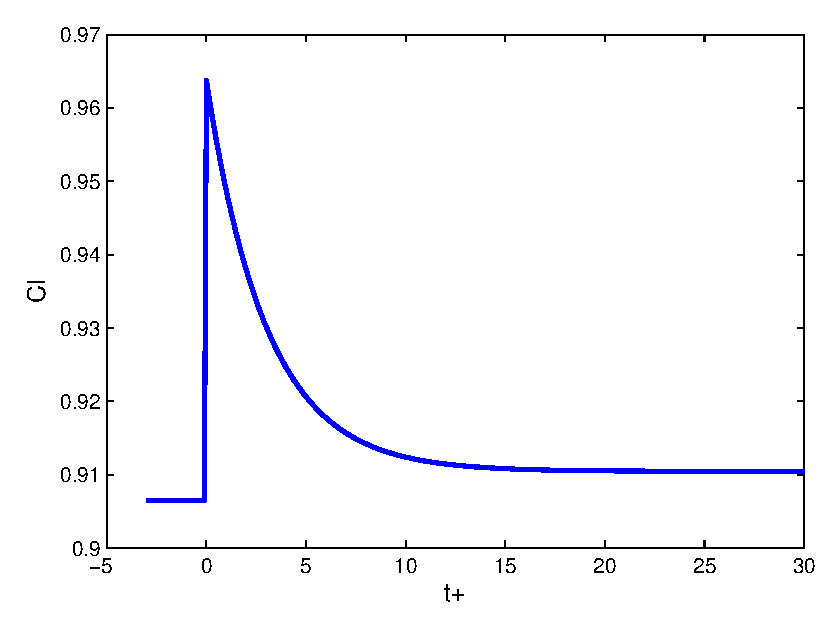
\includegraphics{./Figures/Cl_vs_tplus_step_12to13.eps}
  \caption{Cl behavior for a instantaneous step from 12 to 13 degrees at $t+=0$, as simulated by the GK model}
  \label{fig:Cl_for_alpha_step}
\end{figure}

\FloatBarrier

\par The classical methods used to find the time constant for first order system can be used.
As you can see in the figure \ref{fig:tau_1_identification}, the $\tau_1$ constant found from the GK model output is close to the one used in the model.

\begin{figure}[h]
  \centering
%  \includegraphics{<+file+>}
  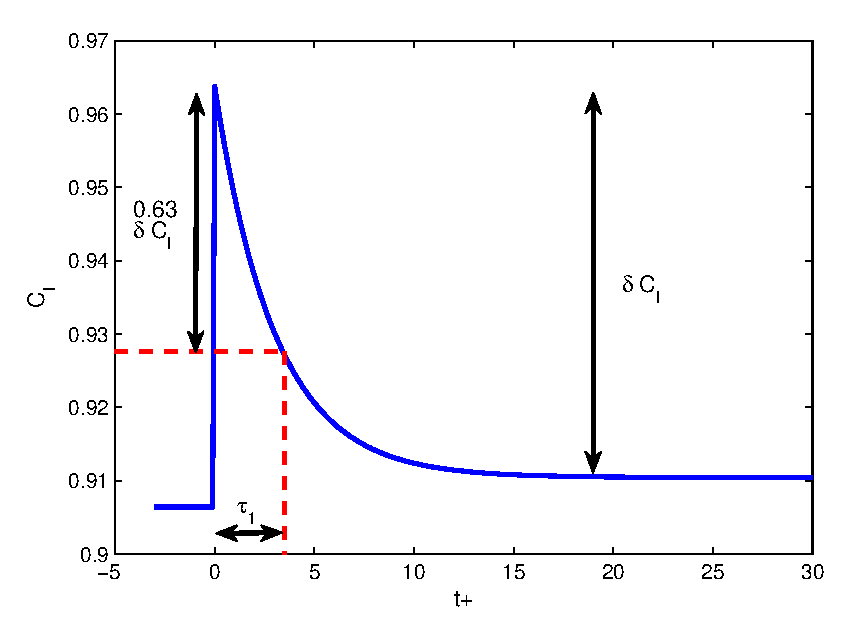
\includegraphics{./Figures/tau_1_Cl_vs_tplus_step_12to13.eps}
  \caption{Identification of $\tau_1$ from the theoretical step response}
  \label{fig:tau_1_identification}
\end{figure}	

\FloatBarrier

\par While this method is fine in theory, it is impossible to implement experimentally.
The force balance used to measure lift and drag is very fragile, so a fast step could be enough to break it.
Furthermore any slower of even smoothed step input modifies the lift response enough to make the time constant identification impossible.
While this method is unpractical for experimental cases it should be applicable in the case of CFD simulations.

\Subsection{Model comparison at different frequencies mean angle and amplitudes}
Now that the model is complete its accuracy can be checked.
The most obvious result is that the shape of the lift and drag versus angle of attack curves are similar to the experimental results.

\begin{figure}[h]
  \begin{center}
    \scalebox{1.0}{
      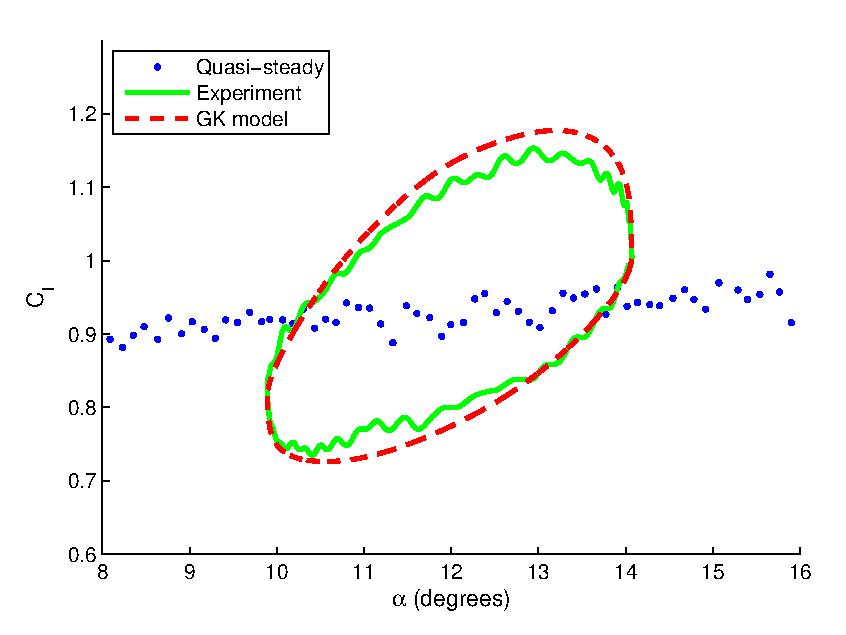
\includegraphics{./Figures/Cl_u=3_meanaoa=12_amp=2_freq=0p5.eps}}
  \end{center}
  \caption{Comparison of experimental lift coefficient and model prediction after tunning of the time constant at k =0.128}
  \label{fig:Cl_u=3_meanaoa=12_amp=2_freq=0p5}
\end{figure}

\begin{figure}[h]
  \begin{center}
    \scalebox{1.0}{
      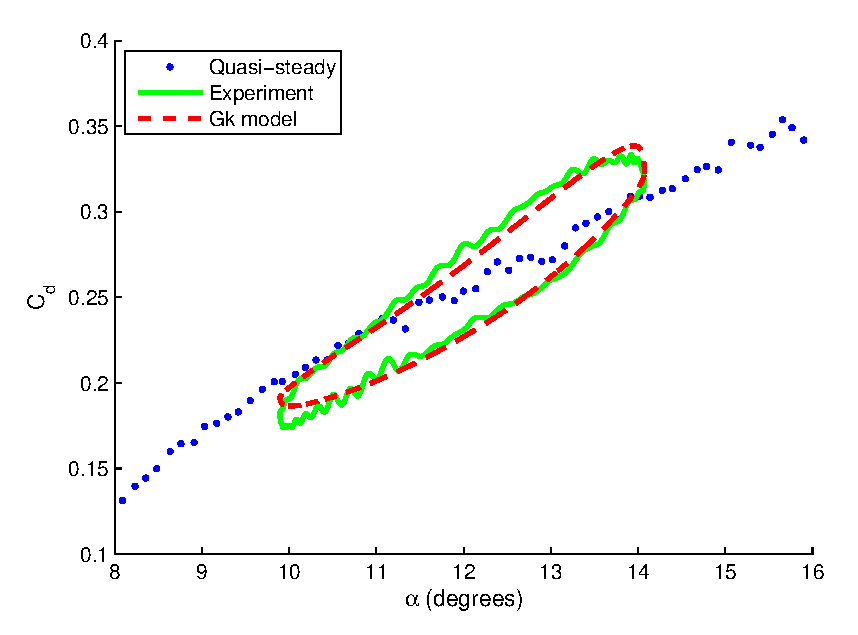
\includegraphics{./Figures/Cd_u=3_meanaoa=12_amp=2_freq=0p5.eps}}
  \end{center}
  \caption{Comparison of experimental drag coefficient and model prediction after tunning of the time constant at k =0.128}
  \label{fig:Cd_u=3_meanaoa=12_amp=2_freq=0p5}
\end{figure}

\FloatBarrier

\par This behavior can be checked for other frequencies as well.

\begin{figure}[h]
  \begin{center}
    \scalebox{1.0}  
    {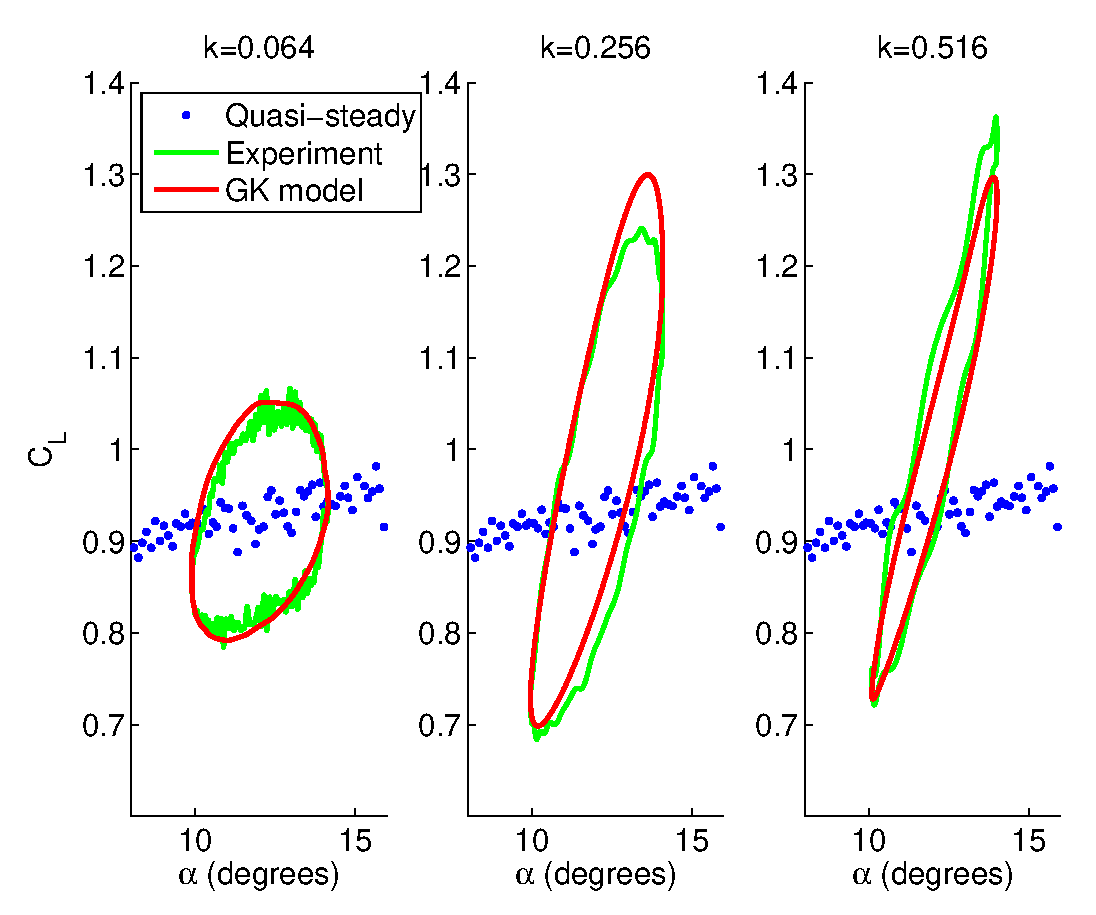
\includegraphics{./Figures/Pitching_allcases_GK_CL_12_amp_2.eps}}
  \end{center}
  \caption{Lift measurement and prediction during sinusoidal pitching around 12 degree} 
  \label{fig:Pitching_allcases_GK_Cl_12}
\end{figure}

\begin{figure}[h]
  \begin{center}
    \scalebox{1.0}  
    {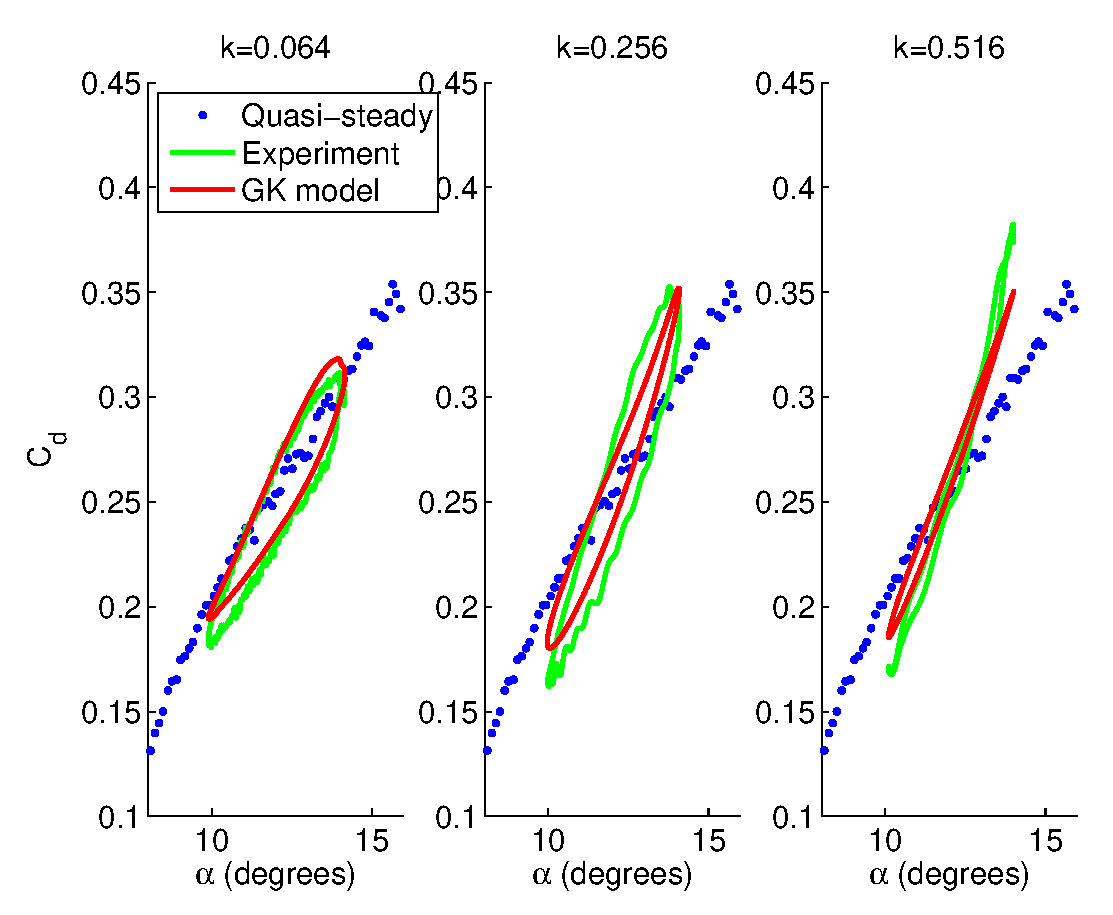
\includegraphics{./Figures/Pitching_allcases_GK_CD_12_amp_2.eps}}
  \end{center}
  \caption{Drag measurement and prediction during sinusoidal pitching around 12 degree} 
  \label{fig:Pitching_allcases_GK_Cd_12}
\end{figure}

\par Similarly another set of acquisitions is made at a mean angle of 10 degrees (see figures \ref{fig:Pitching_allcases_GK_Cl_10} and \ref{fig:Pitching_allcases_GK_Cd_10}).
For some unknown reason the model does not account very well for the behavior of the drag at this frequency.

\begin{figure}[h]
  \begin{center}
    \scalebox{1.0}  
    {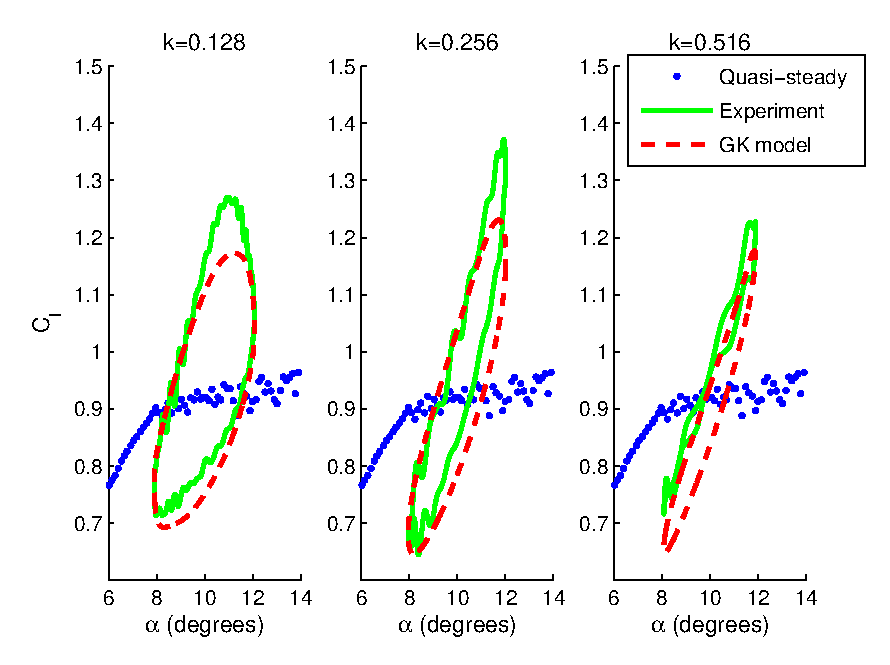
\includegraphics{./Figures/Pitching_allcases_GK_CL_10_amp_2.eps}}
  \end{center}
  \caption{Lift measurement and prediction during sinusoidal pitching around 10 degree} 
  \label{fig:Pitching_allcases_GK_Cl_10}
\end{figure}

\begin{figure}[h]
  \begin{center}
    \scalebox{1.0}  
    {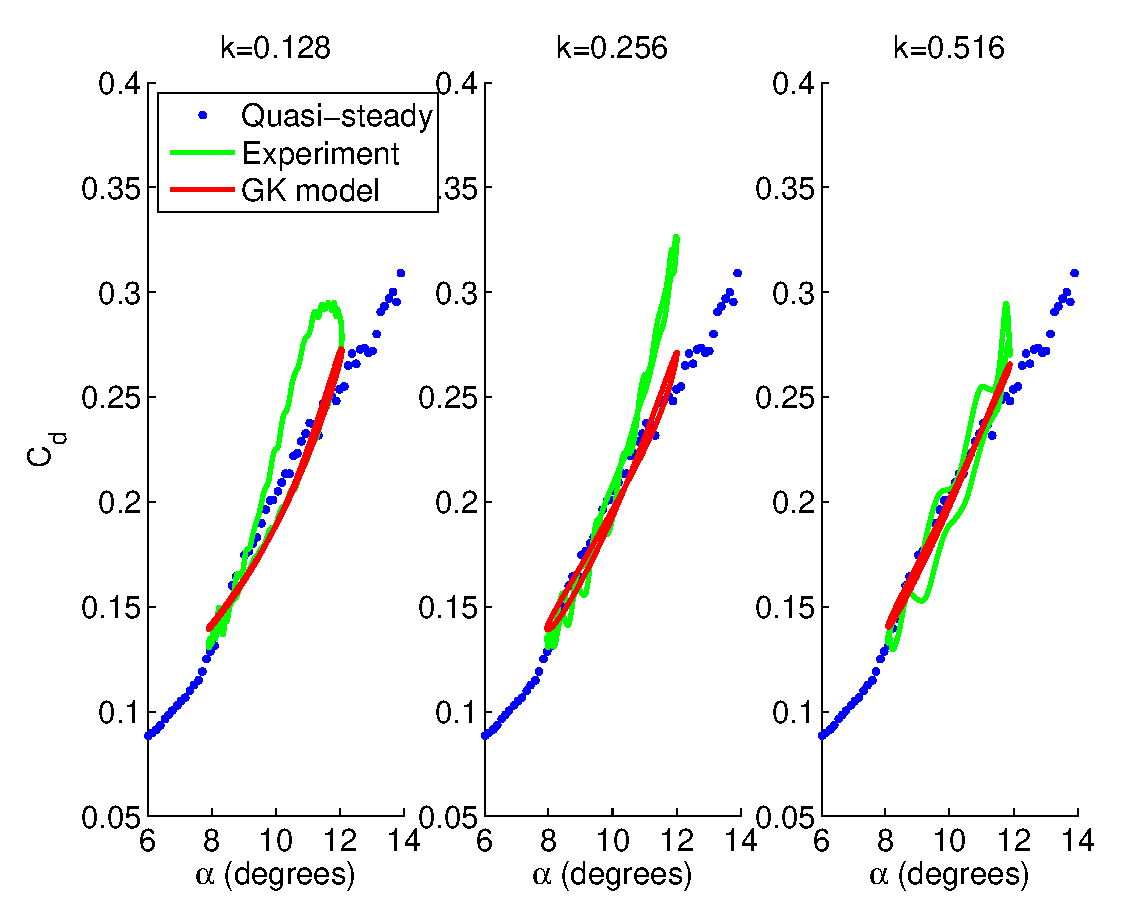
\includegraphics{./Figures/Pitching_allcases_GK_CD_10_amp_2.eps}}
  \end{center}
  \caption{Drag measurement and prediction during sinusoidal pitching around 10 degree} 
  \label{fig:Pitching_allcases_GK_Cd_10}
\end{figure}

\FloatBarrier

\emph{GRAPH FOR THIS IS NEEDED!!!}

\par The area around 8 degrees is interesting, because this is where the flow just starts to become separated.
The transition between attached flow and separated flow means that the state variable $x$ should not have any effect for the lower angles and as a consequence the loop seen in the $C_l$ versus $\alpha$ plots should be ``pinched'' on its left side.
This can be further illustrated by plotting the value of the state variable during this kind of maneuvers, it is constrained by the saturation of this value at one.
This kind of behavior is particularly apparent on high amplitude (tens of degrees) pitch maneuver as it is seen in the original Goman and Khrabrov paper.
The behavior is comparable at $k$ of 0.257 and 0.513 but the drag has a noticeably different shape at $k$ of 0.128.

\par Another obvious parameter to check for our model is the amplitude of the oscillations.
The amplitude is set to a range from 1 to 4 degrees at different mean angle of attack.
The predictions still reasonably match the experimental results. 

% divers figures

\Subsection{Non-periodic pitch input}
To simulate a more realistic pitch profile, a pseudo-random pitch profile is designed.
The input is constructed as seen in equation \ref{eqn:random_pitch_input} with a randomized phase difference $\varphi_i$ between each of the harmonic components.

\begin{equation}
	\alpha_{random}= \frac{\sum_{i=1}^{10} \sin (\frac{2 \pi t}{f_i} + \varphi_i)}{B} + \alpha_{0}
	\label{eqn:random_pitch_input}
\end{equation}

The frequencies regularly spaced between 0.25 and 2 Hz and the constant $B$ is chosen to make sure the maximum deviation from the $\alpha_0$ value is no more than 2 degrees.
This is done so that the bandwidth of the input signal is limited to reasonable levels and to keep the force balance safe.

\begin{figure}[h]
  \begin{center}
    \scalebox{1.0}  
  {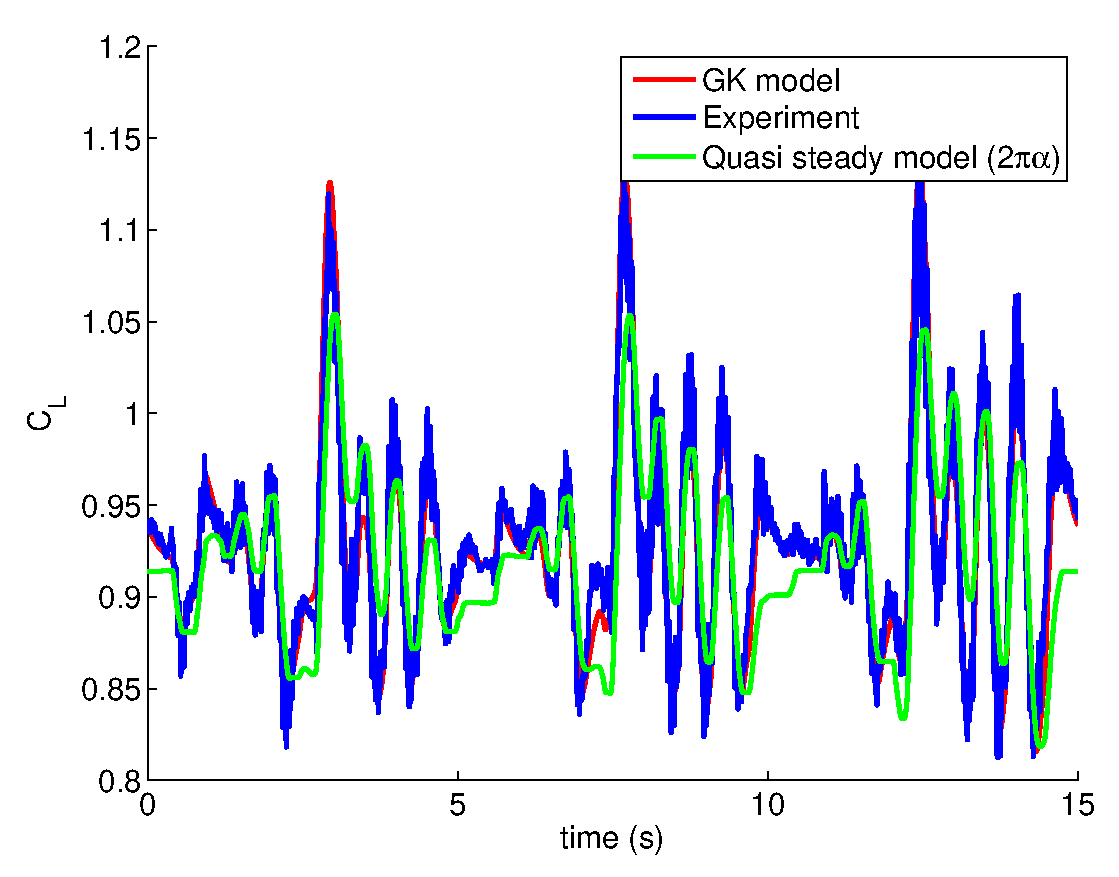
\includegraphics{./Figures/Cl_u=3_meanaoa=12(15seconds)_amp=2_freq=2p0.eps}}
  \end{center}
  \caption{Unsteady effects of random pitching on the lift}
  \label{fig:Pitching_random_Cl_12}
\end{figure}

\begin{figure}[h]
  \begin{center}
    \scalebox{1.0}  
  {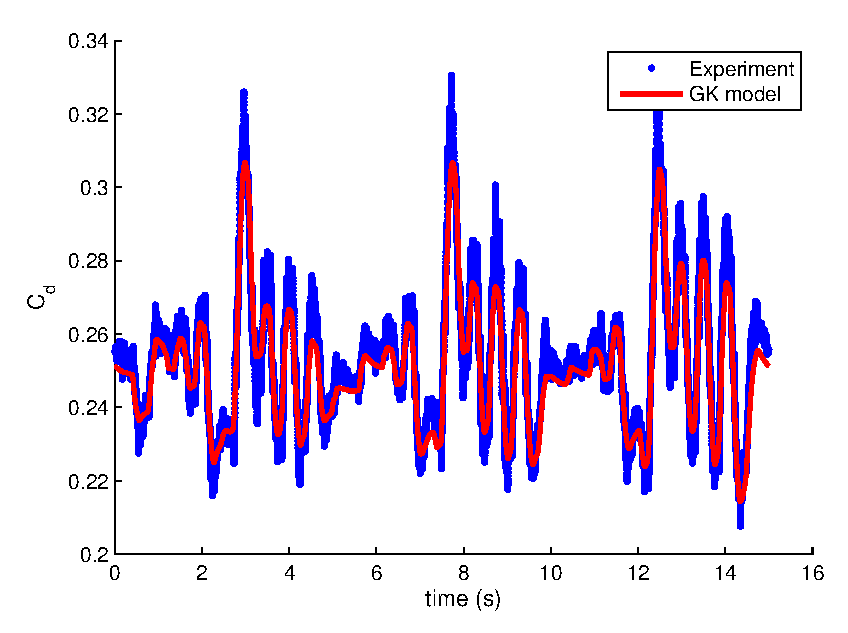
\includegraphics{./Figures/Cd_u=3_meanaoa=12(15seconds)_amp=2_freq=2p0.eps}}
  \end{center}
  \caption{Unsteady effects of random pitching on the drag}
  \label{fig:Pitching_random_Cd_12}
\end{figure}

\par The accuracy of these results means that this model could be used in real time during arbitrary pitching maneuvers.
This is potentially very useful since a lot of systems rely on the periodicity of the pitching motion to predict the lift and can be inaccurate in case of non periodic disturbances such as wind gusts changing the effective angle of attack.

\FloatBarrier

\par This model is producing accurate results that account for both the dynamic effects and the flow separation.
Moreover the procedure is simple enough to be implemented into the optimization algorithm without increasing too much the computation cost.


\Section{Model limitations}

While this model produces impressive results for a lot of different cases, it is not without its limitations.

\Subsection{Inertial and added mass effects} \label{subs:added_mass}
One of the biggest issues of the experimental part for the pitching experiment are the inertial effects due to the mass of the wing.
These inertial effects represent very high loads compared to the actual aerodynamic loads.
To measure the inertial effects we get the weight of the wing being added to the force balance measurement.

\par Since we are only interested in the aerodynamic forces, we need to eliminate these mechanical forces.
As explained before we remove these by averaging over several cycles both an acquisition with the tunnel on and one without the model on.
Assuming that the inertial effects are reproducible (this has been a fairly solid assumption) then the forces due to the momentum and weight are removed.
However the acquisition done when the wind tunnel is not running are not done in vacuum.
As such the added mass effects are also subtracted from the final data.

\Subsection{Center of rotation}
Traditionally whenever span-wise data are considered, all moments and rotation centers are taken at the quarter chord point.
With our double servomotor system we are able to find a relation which will allow us to rotate the wing around any arbitrary point (provided it is within the mechanical range of the actuators).
A batch of measurements was performed with the rotation point set at the location of the force balance to minimize the effects of the inertial tangential and normal forces on the measurements.
However the results were deemed not as good as simply moving the rear servo.
The simultaneous motion of the two servos introduce a lot of vibrations, especially when small and slow motions are needed.
This is due to the electric servos being based on stepper motors and the fact that the two servo rods are very close together.

\par Attempts to move only the back servo (instead of the front) produced worst data than moving the back one.
A possible explanation is that the front servo has to support the whole wing and sting assembly whereas the back one has a much lighter load.
Under the higher load the servo positioning system is not as precise.

\par Any unwanted forces created by rotating the airfoil in front of the quarter chord point should be subtracted by the procedure described in the previous section \ref{subs:added_mass}.
